
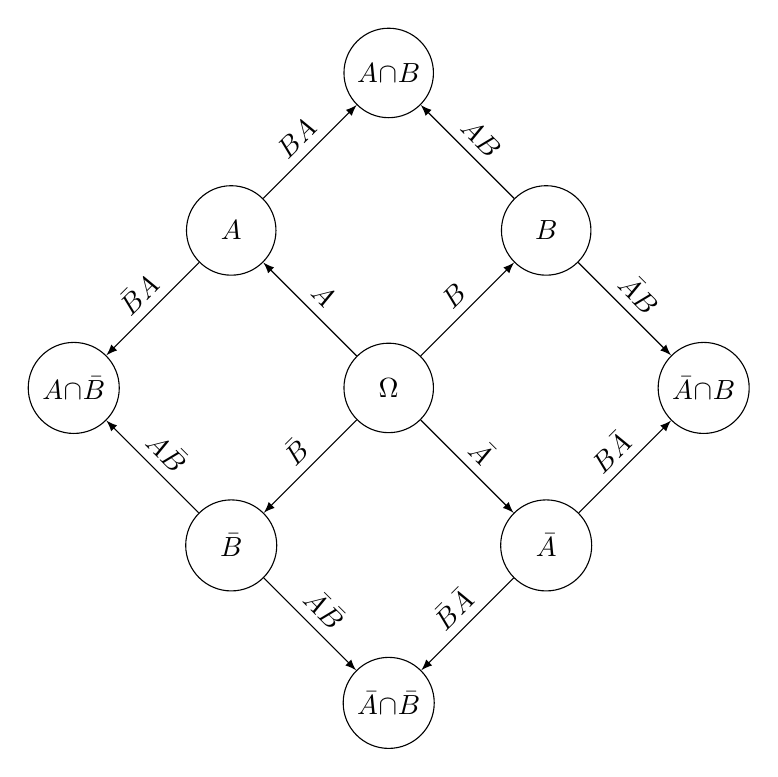
\begin{tikzpicture}[circlenode/.style={draw,circle,text width=0.8cm,align=center}]
  %\draw[help lines] (-3,-3) grid (3,3);


  \draw ( 0, 0) node[circlenode](O) {$\Omega$};

  \draw (-2, 2) node[circlenode](A)     {$A$};
  \draw ( 2, 2) node[circlenode](B)     {$B$};
  \draw ( 2,-2) node[circlenode](bA)    {$\bar{A}$};
  \draw (-2,-2) node[circlenode](bB)    {$\bar{B}$};

  \draw ( 0, 4) node[circlenode](AnB)     {$A\cap B$};
  \draw (-4, 0) node[circlenode](AnbB)    {$A\cap \bar{B}$};
  \draw ( 4, 0) node[circlenode](bAnB)    {$\bar{A}\cap B$};
  \draw ( 0,-4) node[circlenode](bAnbB)   {$\bar{A}\cap \bar{B}$};

  \draw[-latex] (O) -- (A)  node [midway,above,sloped] {$\Prob{A}$};
  \draw[-latex] (O) -- (B)  node [midway,above,sloped] {$\Prob{B}$};
  \draw[-latex] (O) -- (bA) node [midway,above,sloped] {$\Prob{\bar{A}}$};
  \draw[-latex] (O) -- (bB) node [midway,above,sloped] {$\Prob{\bar{B}}$};

  \draw[-latex] (A) -- (AnB)  node [midway,above,sloped] {$\Probc{B}{A}$};
  \draw[-latex] (A) -- (AnbB)  node [midway,above,sloped] {$\Probc{\bar{B}}{A}$};

  \draw[-latex] (bA) -- (bAnB)  node [midway,above,sloped] {$\Probc{B}{\bar{A}}$};
  \draw[-latex] (bA) -- (bAnbB)  node [midway,above,sloped] {$\Probc{\bar{B}}{\bar{A}}$};

  \draw[-latex] (B) -- (AnB)  node [midway,above,sloped] {$\Probc{A}{B}$};
  \draw[-latex] (B) -- (bAnB)  node [midway,above,sloped] {$\Probc{\bar{A}}{B}$};

  \draw[-latex] (bB) -- (AnbB)  node [midway,above,sloped] {$\Probc{A}{\bar{B}}$};
  \draw[-latex] (bB) -- (bAnbB)  node [midway,above,sloped] {$\Probc{\bar{A}}{\bar{B}}$};


\end{tikzpicture}

